
\chapter{Dokumentace}\label{kap:dokumentace}

Tato kapitola je věnovaná dokumentaci, konkrétně uživatelské (\autoref{sec:user-docs}), vývojářské (\autoref{sec:developer-docs}) a administrátorské (\autoref{sec:admin-docs}). Dokumentace je také dostupná online na \url{https://bliakher.github.io/uredni_desky_docs/} a jako příloha \ref{sub:repo2}.

\section{Uživatelská dokumentace}\label{sec:user-docs}


V navigačním panelu aplikace najdeme odkazy do 4 částí aplikace: 
\begin{itemize}
    \item Seznam \autoref{seznam}
    \item Mapa \autoref{mapa}
    \item Statistiky \autoref{statistiky}
    \item Validace \autoref{validace}
\end{itemize}

\subsection*{Seznam}\label{seznam}

\begin{figure}
\centering
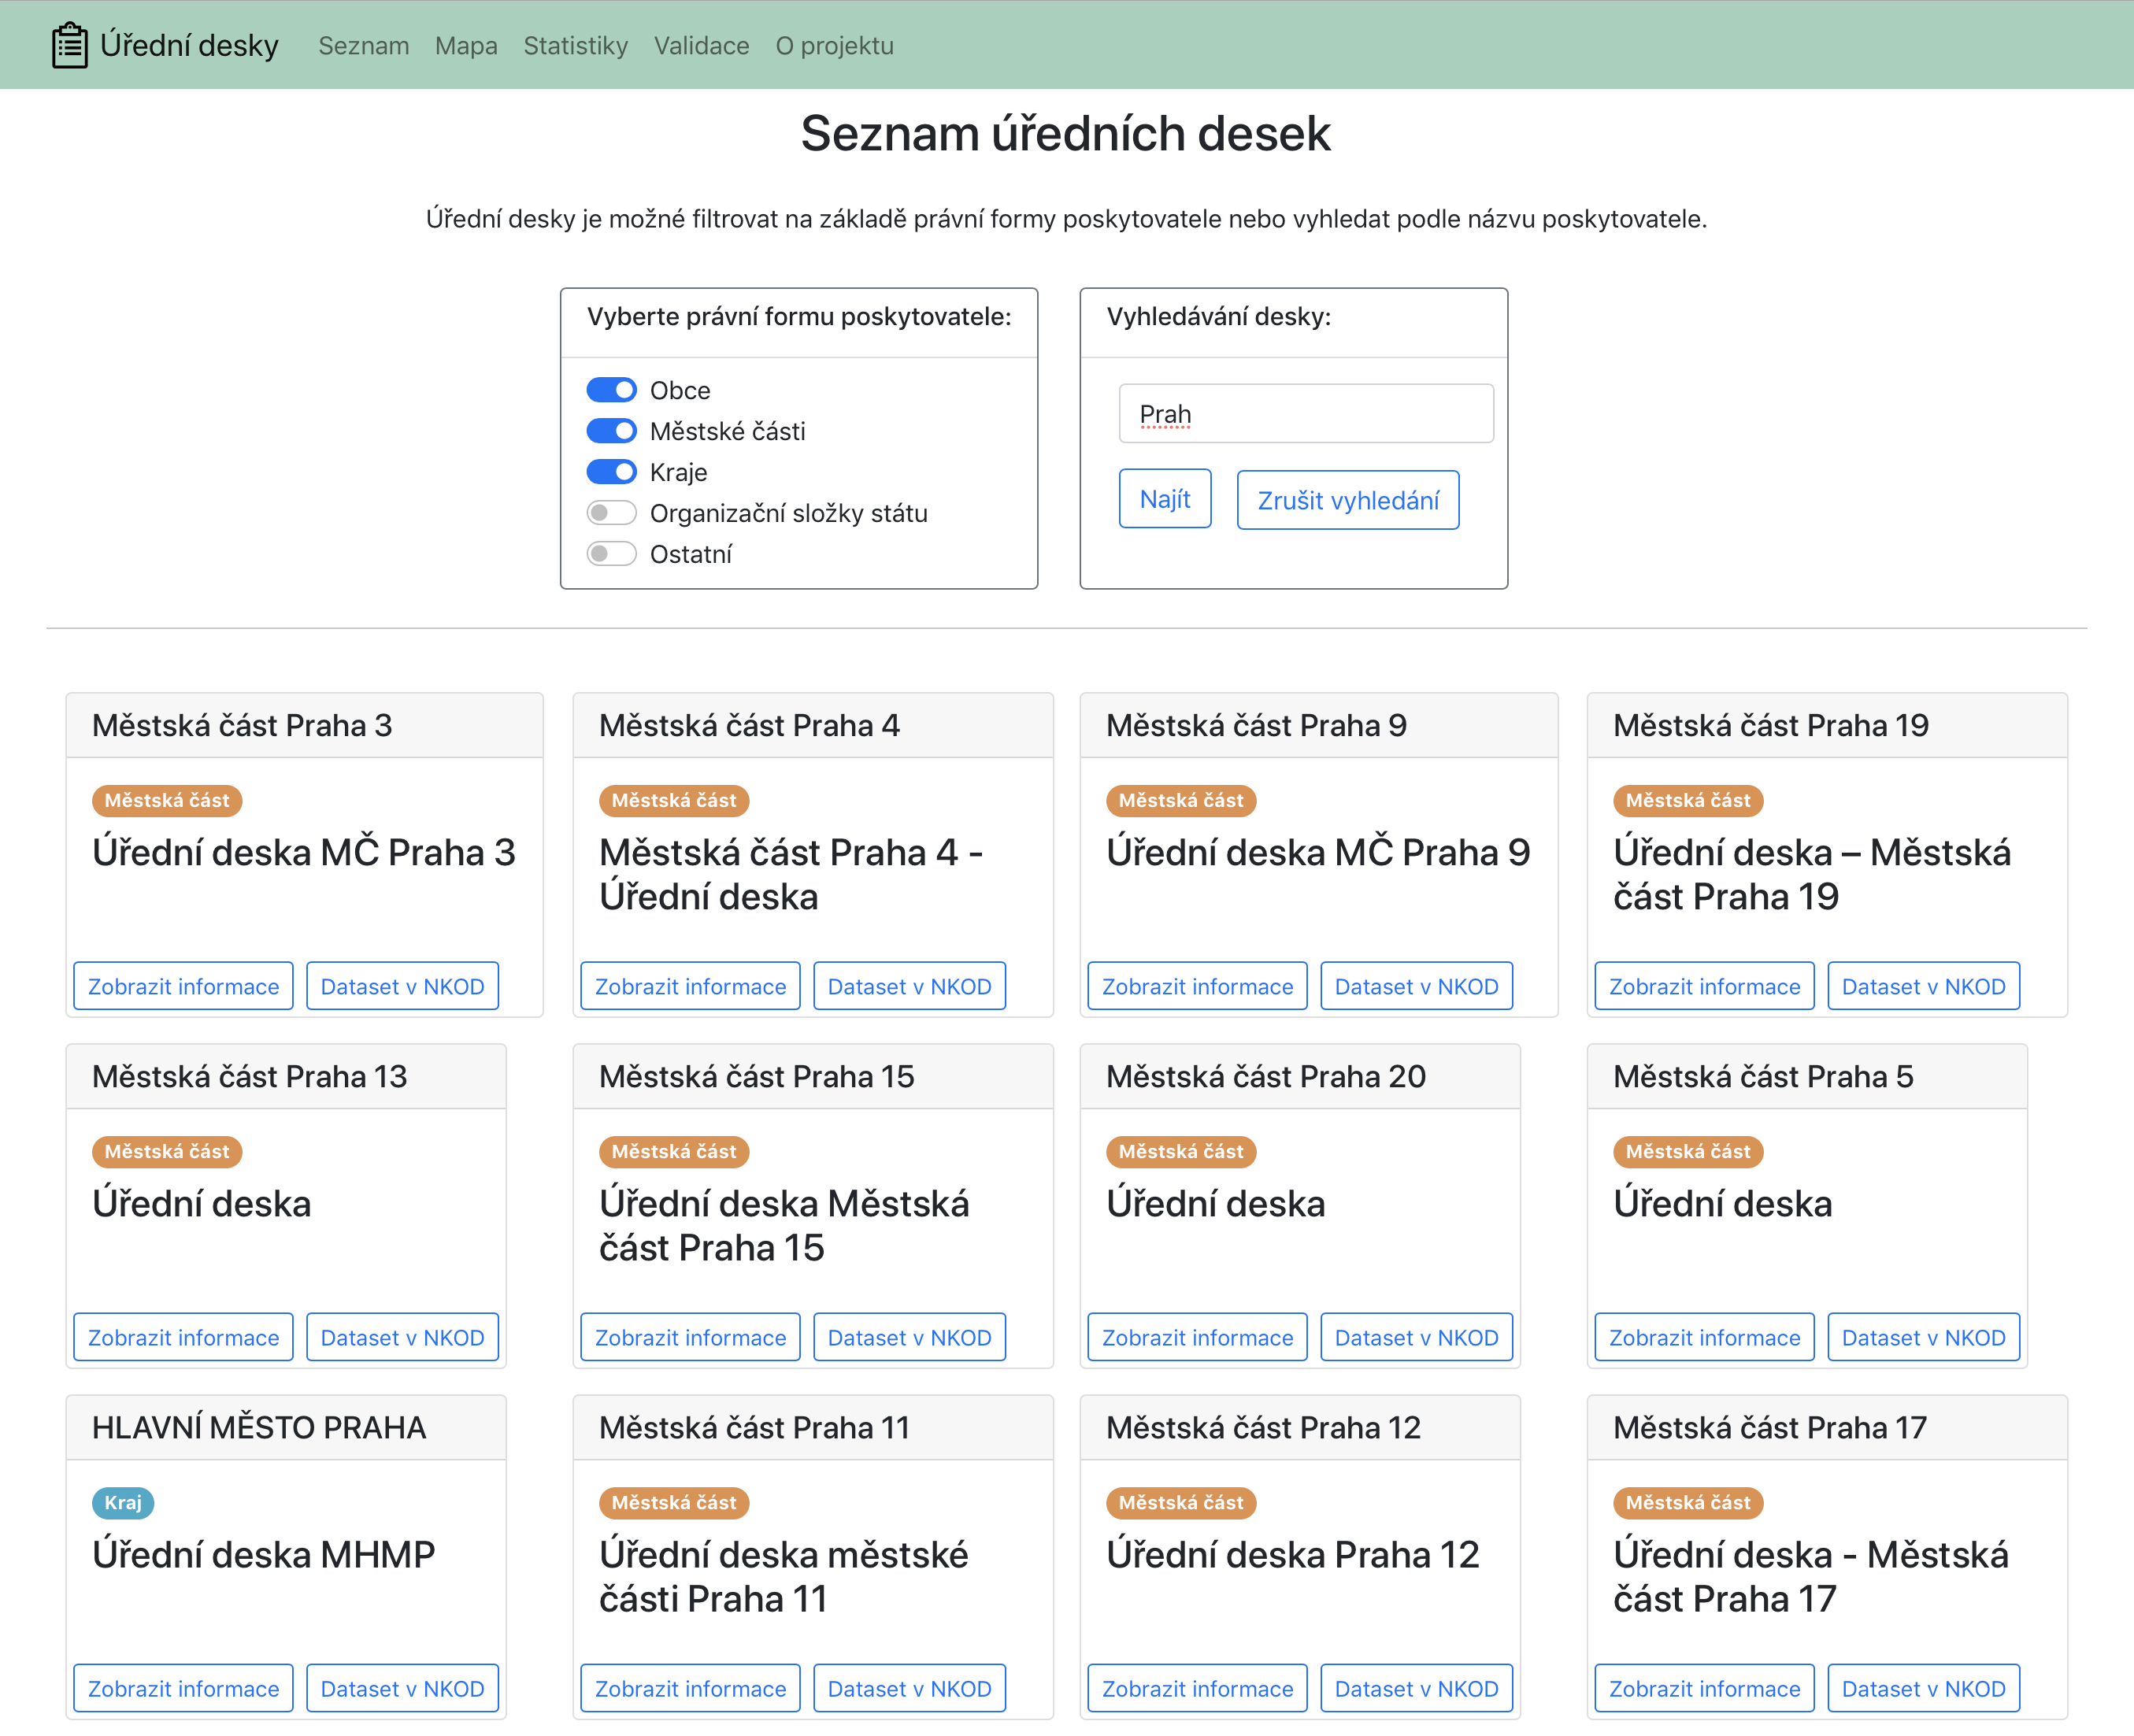
\includegraphics[width=\textwidth]{cs/obrazky/screenshots/seznam.png}
\caption{Ukázka filtrování v seznamu úředních desek}
\label{fig:screen-seznam}
\end{figure}

Tato část obsahuje seznam všech úředních desek, které má aplikace k
dispozici. Aplikace data z úředních desek získává z Národního katalogu
otevřených dat (NKOD), může tedy zobrazit pouze ty desky, které jsou
daným úřadem zveřejněné v NKOD jako otevřená data.

Úřední desky je možné filtrovat podle právní formy poskytovatele. Právní
formy, které podporujeme jsou: 
\begin{itemize}
    \item obce
    \item městské části a městské obvody
    \item kraje
    \item organizační složky státu
\end{itemize}

Právní formy poskytovatelů zjišťujeme z údajů uvedených v
\href{https://www.szrcr.cz/cs/registr-prav-a-povinnosti}{Registru práv a
povinností}. Poskytovatelé ostatních právních forem, nebo poskytovatelé,
u kterých nelze zjistit formu jsou v kategorii ostatní.

Pro filtrování desek použijte panel
\textit{Vyberte\ právní\ formu\ poskytovatele}. Nechte vybrané pouze ty
právní formy, jejichž poskytovatele chcete vyfiltrovat.

V úředních deskách je také možné vyhledávat na základě názvu desky nebo
jména poskytovatele pomocí formuláře pro vyhledávání.

Na obrázku \ref{fig:screen-seznam} je příklad seznamu, kde jsou vyfiltrované pouze úřední desky týkající se
Prahy od poskytovatelů s právními formami obec, městská část nebo kraj.

Ze seznamu je možné přejít na detail úřední desky zmáčknutím tlačítka \\
\textit{Zobrazit\ informace}. V detailu desky se zobrazují informace z
dané úřední desky, ve kterých je možné vyhledávat podle názvu s použitím
formuláře na vyhledávání.

\begin{figure}
\centering
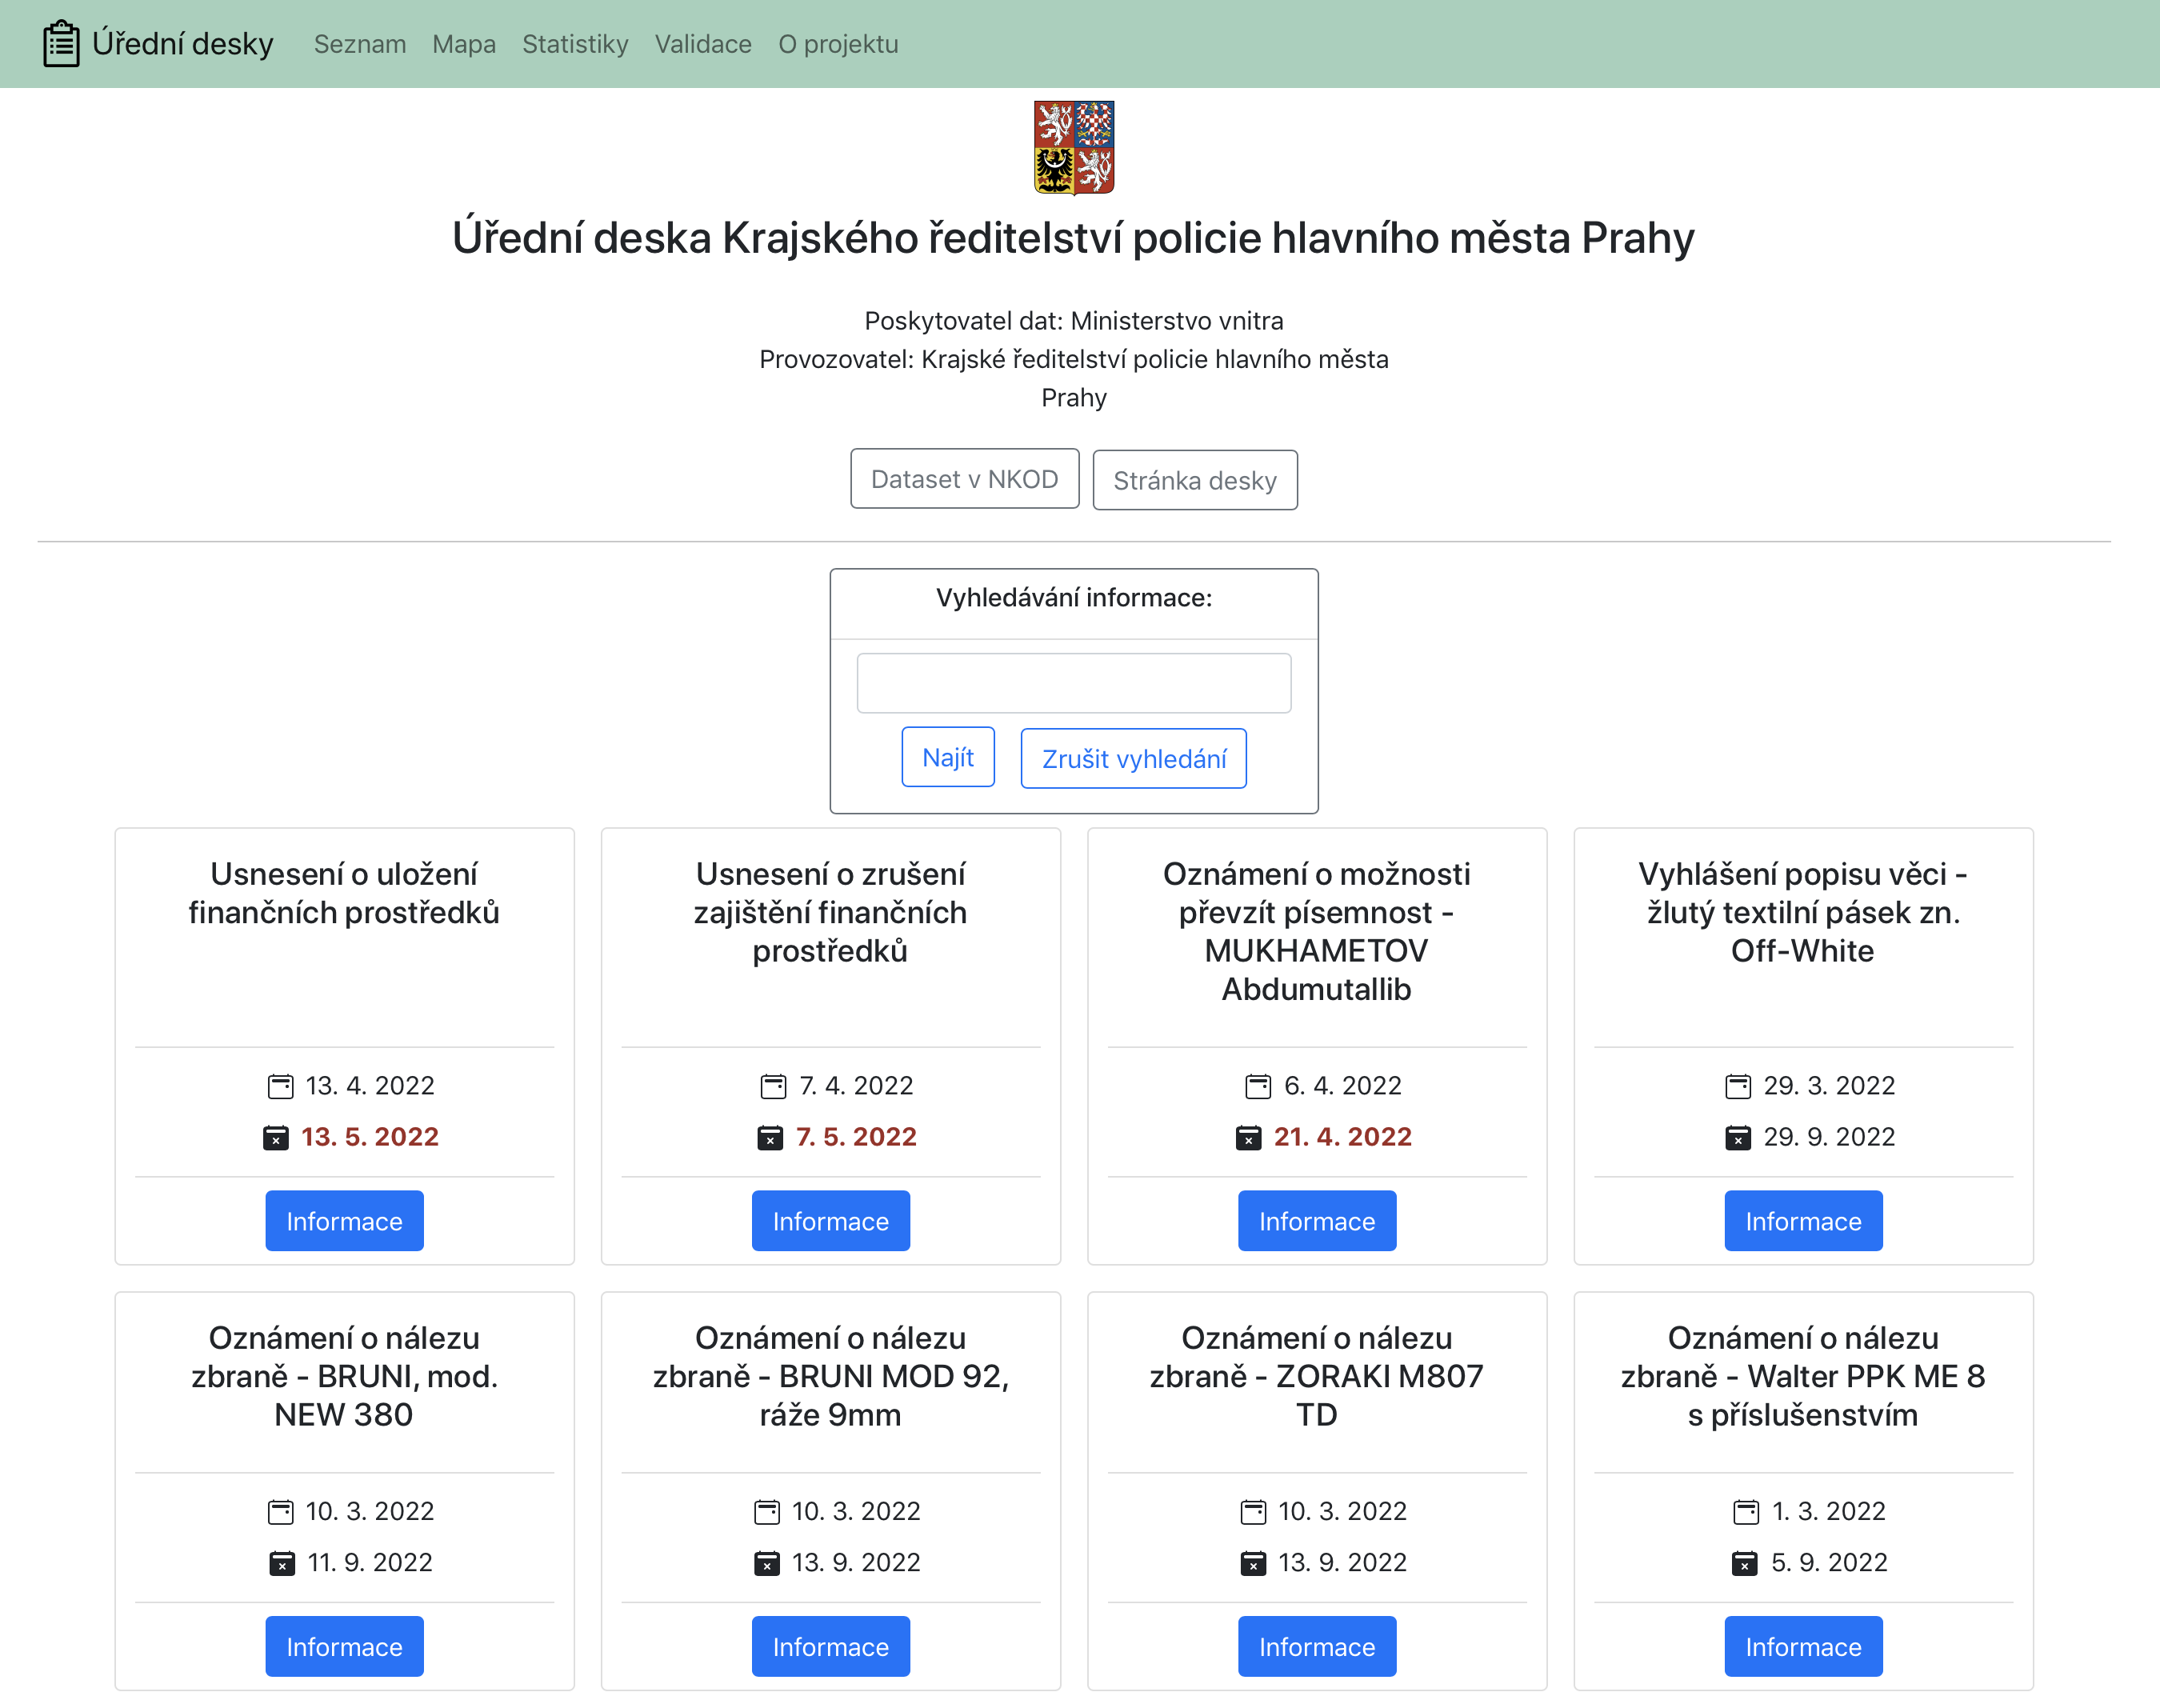
\includegraphics[width=\textwidth]{cs/obrazky/screenshots/detail.png}
\caption{Ukázka detailu úřední desky}
\label{fig:screen-detail}
\end{figure}

Na obrázku \ref{fig:screen-detail} vidíme příklad detailu úřední desky Krajského ředitelství policie
hl. m. Prahy. Pokud informace na desce již není relevantní, tedy datum relevance již
uplynulo, je datum zvýrazněné červeně.

\subsection*{Mapa}\label{mapa}

V této části jsou úřední desky zobrazené na mapě ČR. Úřední desky jsou
rozdělené podle poskytovatelů, kteří zveřejnili data v NKOD.
Poskytovatel je na mapě označen bodem, který je zbarvený podle právní
formy poskytovatele. Legenda k barvám je umístěná nad mapou.

Při kliknutí na bod na mapě se pod mapou zobrazí název daného
poskytovatele a všechny jeho úřední desky. Ze seznamu desek je opět
možné přejít do detailu desky.

Příklad zobrazení desky úřadu městské části Praha 13 z mapy je na obrázku \ref{fig:screen-mapa}.

\begin{figure}
\centering
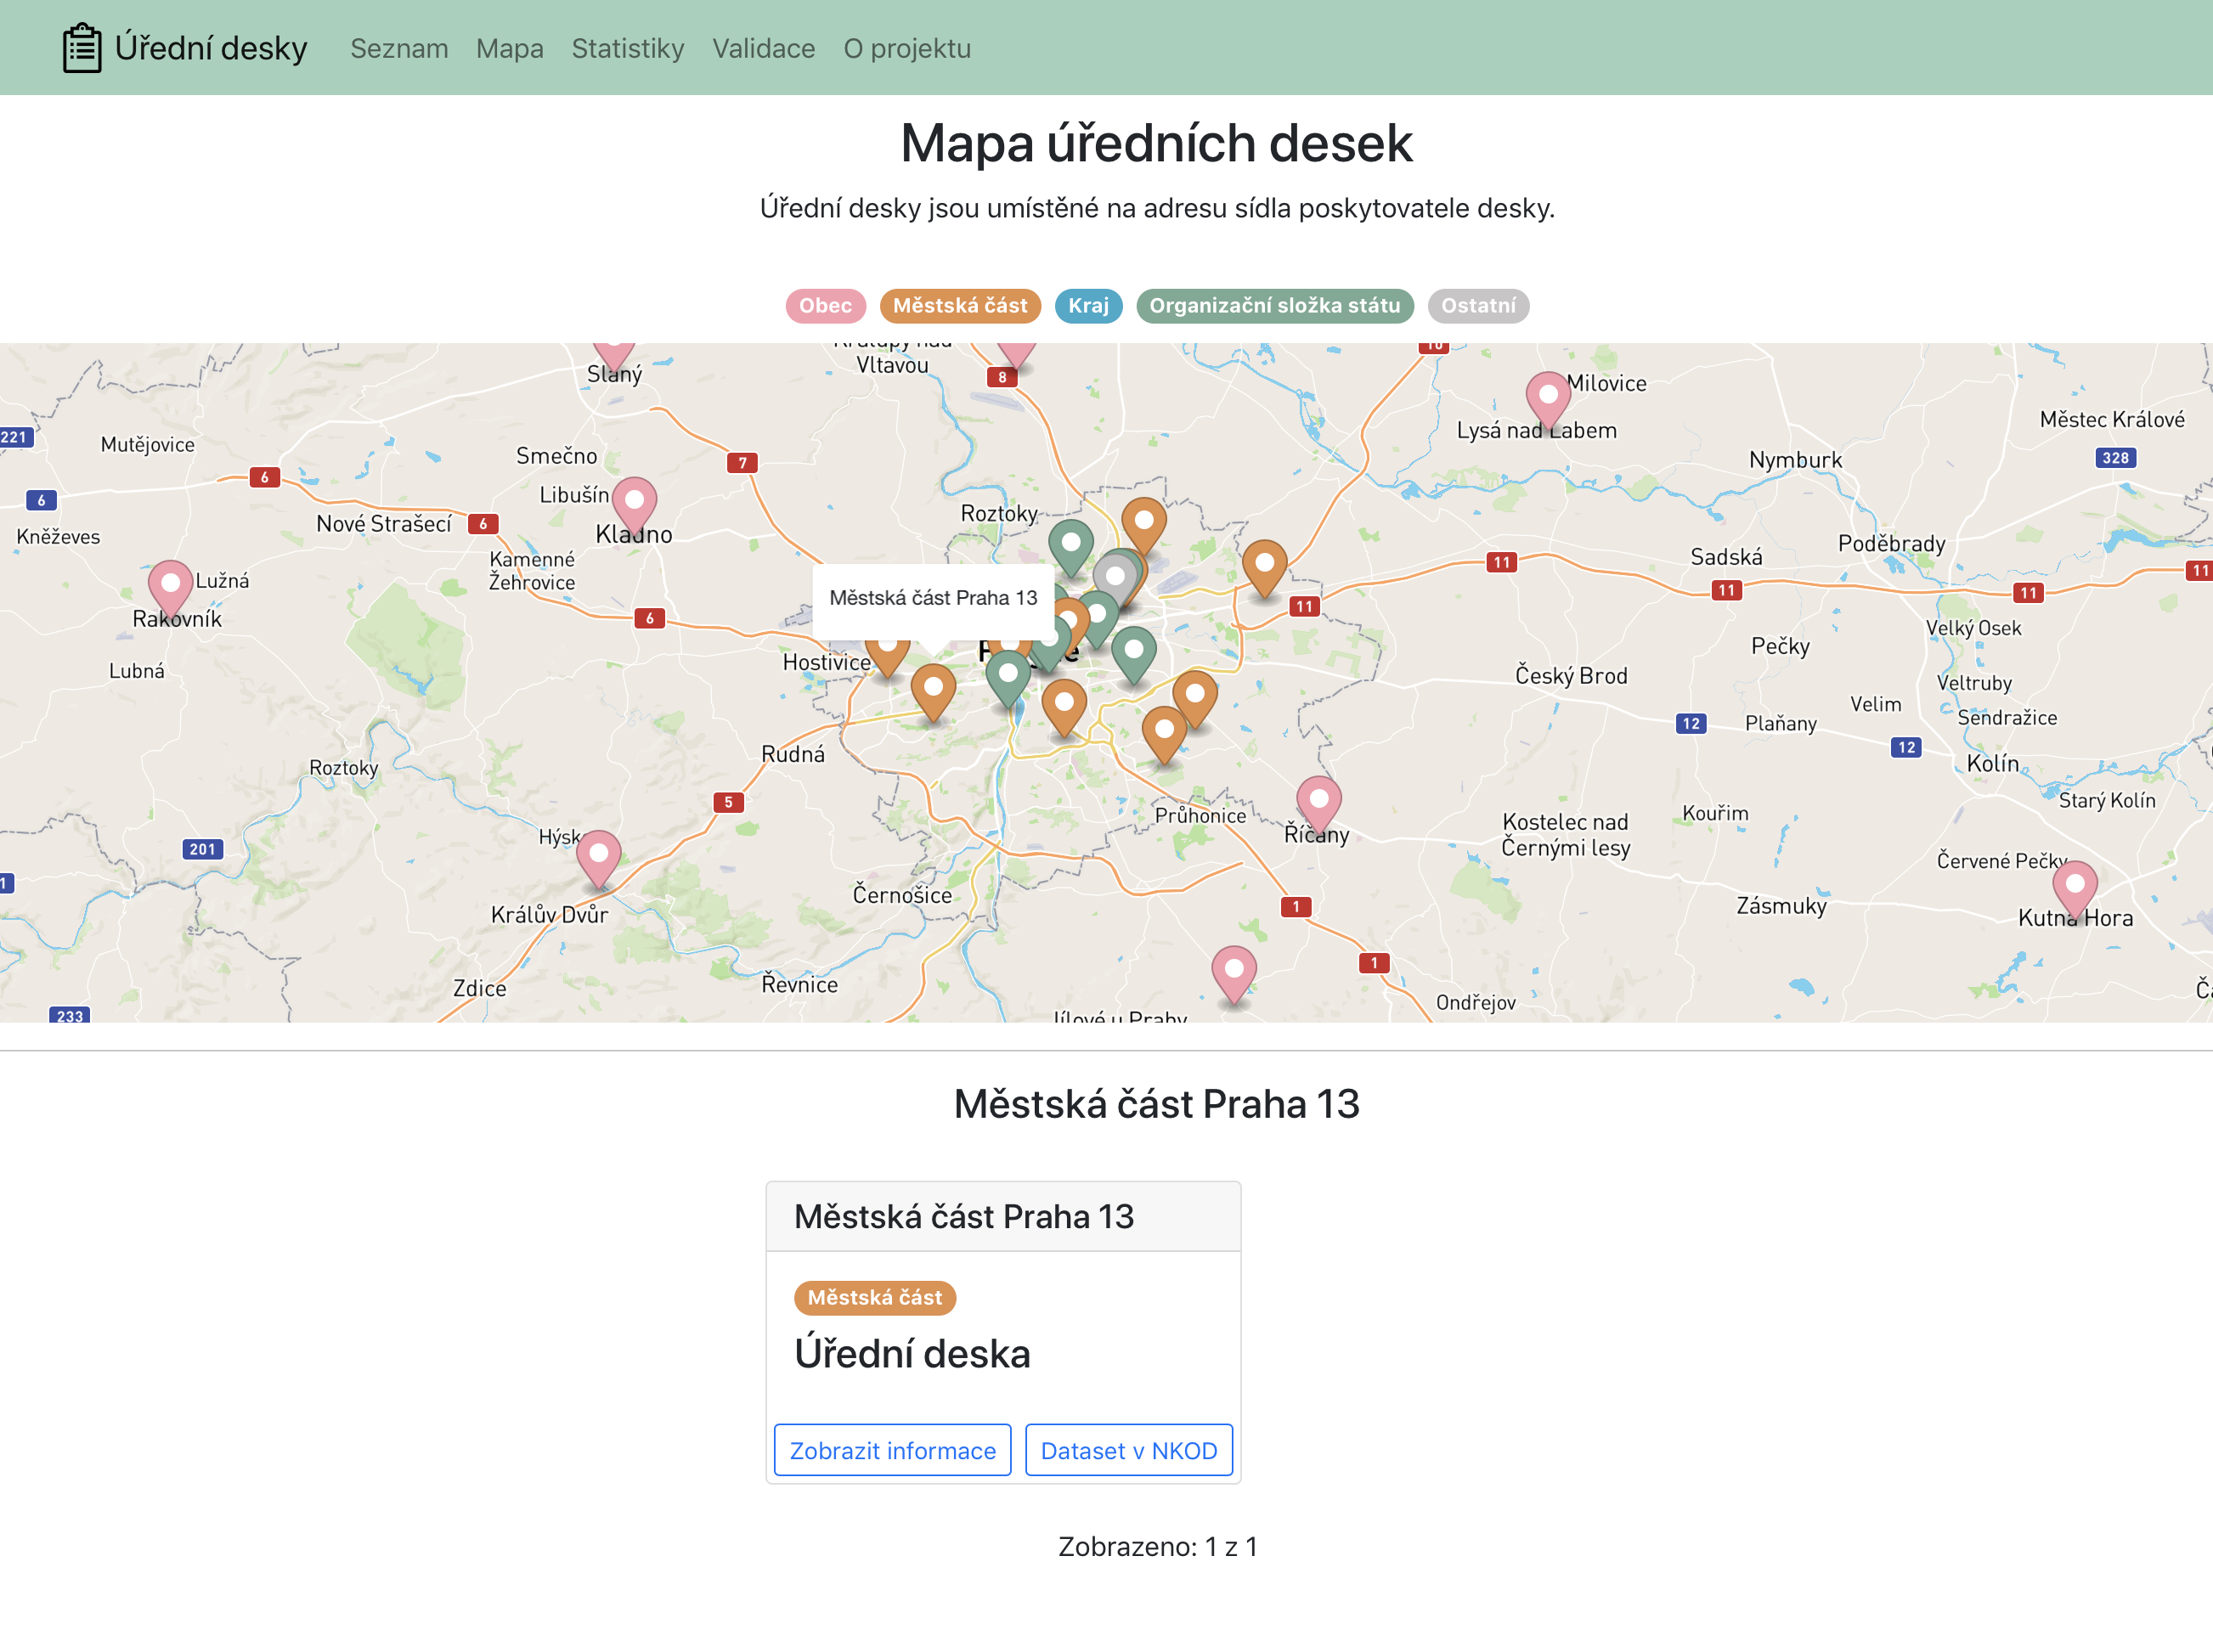
\includegraphics[width=\textwidth]{cs/obrazky/screenshots/mapa.png}
\caption{Ukázka zobrazení desky úřadu městské části Praha 13 na mapě}
\label{fig:screen-mapa}
\end{figure}

\subsection*{Validace}\label{validace}

Část validace je určená hlavně poskytovatelům dat. Provádí se zde
validace dat, konkrétně se kontroluje, jestli je data možné stáhnout a
jestli obsahují všechny doporučené parametry podle specifikace datového
formátu, podle kterého se mají zveřejňovat, který je určený
\href{https://ofn.gov.cz/úřední-desky/2021-07-20/}{Otevřenou formální
normou pro úřední desky}.

Výsledky validace jsou znázorněné tabulkou. Každý řádek tabulky
představuje shrnutí výsledků validace jedné úřední desky. Řádek obsahuje
název desky a jejího poskytovatele, informaci o tom, jestli je možné
stáhnout distribuci s daty desky, jestli data obsahují všechny
doporučené atributy a počet informací na desce.

Na obrázku \ref{fig:screen-validace} je příklad tabulky s výsledky validace, kde jsou vyfiltrované pouze
úřední desky městských částí. Pro větší přehlednost jsou řádky s deskou,
kde není možné stáhnout distribuci, obarvené červeně, a řádky desek, kde
chybí některé doporučené atributy, jsou obarvené žlutě.

\begin{figure}
\centering
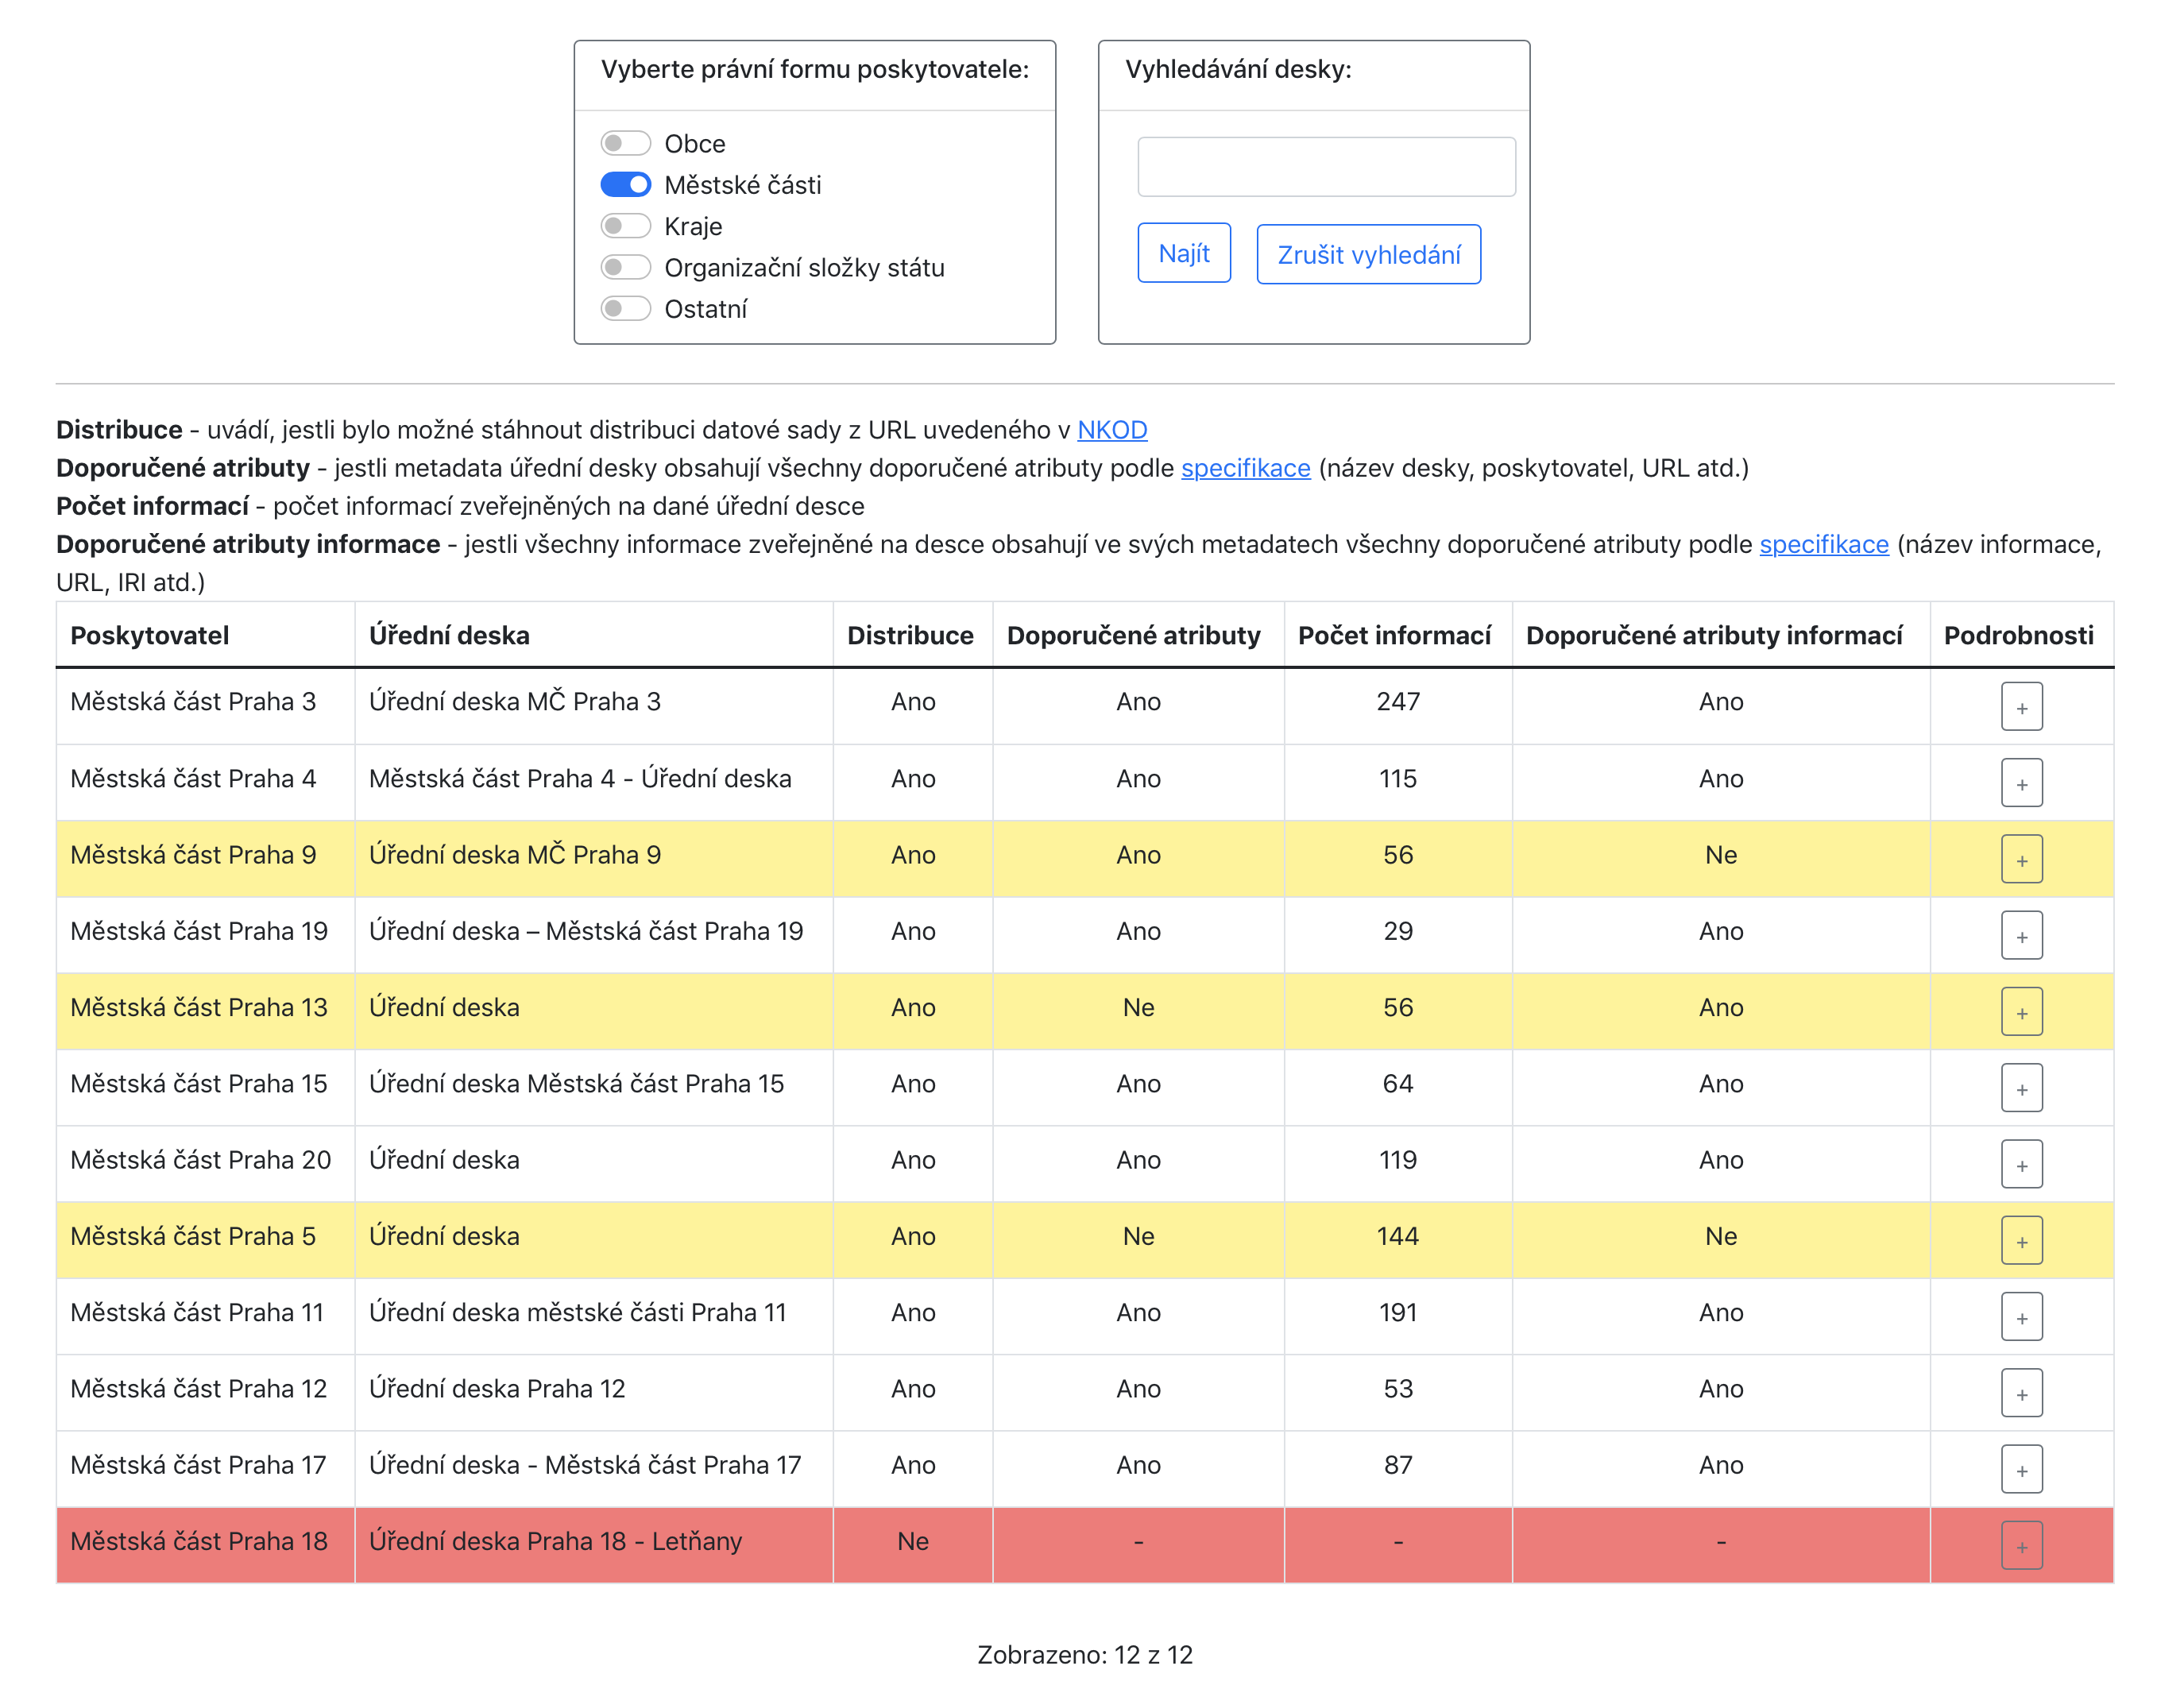
\includegraphics[width=\textwidth]{cs/obrazky/screenshots/validace.png}
\caption{Ukázka validace úředních desek poskytovatelů s právní formou městská část}
\label{fig:screen-validace}
\end{figure}

Z tabulky je možné se prokliknout na detail validace. Je zde vysvětleno,
jakým způsobem se validuje a jaký je význam jednotlivých doporučených
atributů (v části \textit{Jak\ validujeme?}).

Pokud distribuci desky není možné stáhnout, zobrazí se v detailu chybová
hláška získaná při stahování a seznam nejčastějších příčin, které tento
problém způsobují s odkazy na další informace o problému jako vidíme na
další ukázce, \autoref{fig:screen-validace-c}.

\begin{figure}
\centering
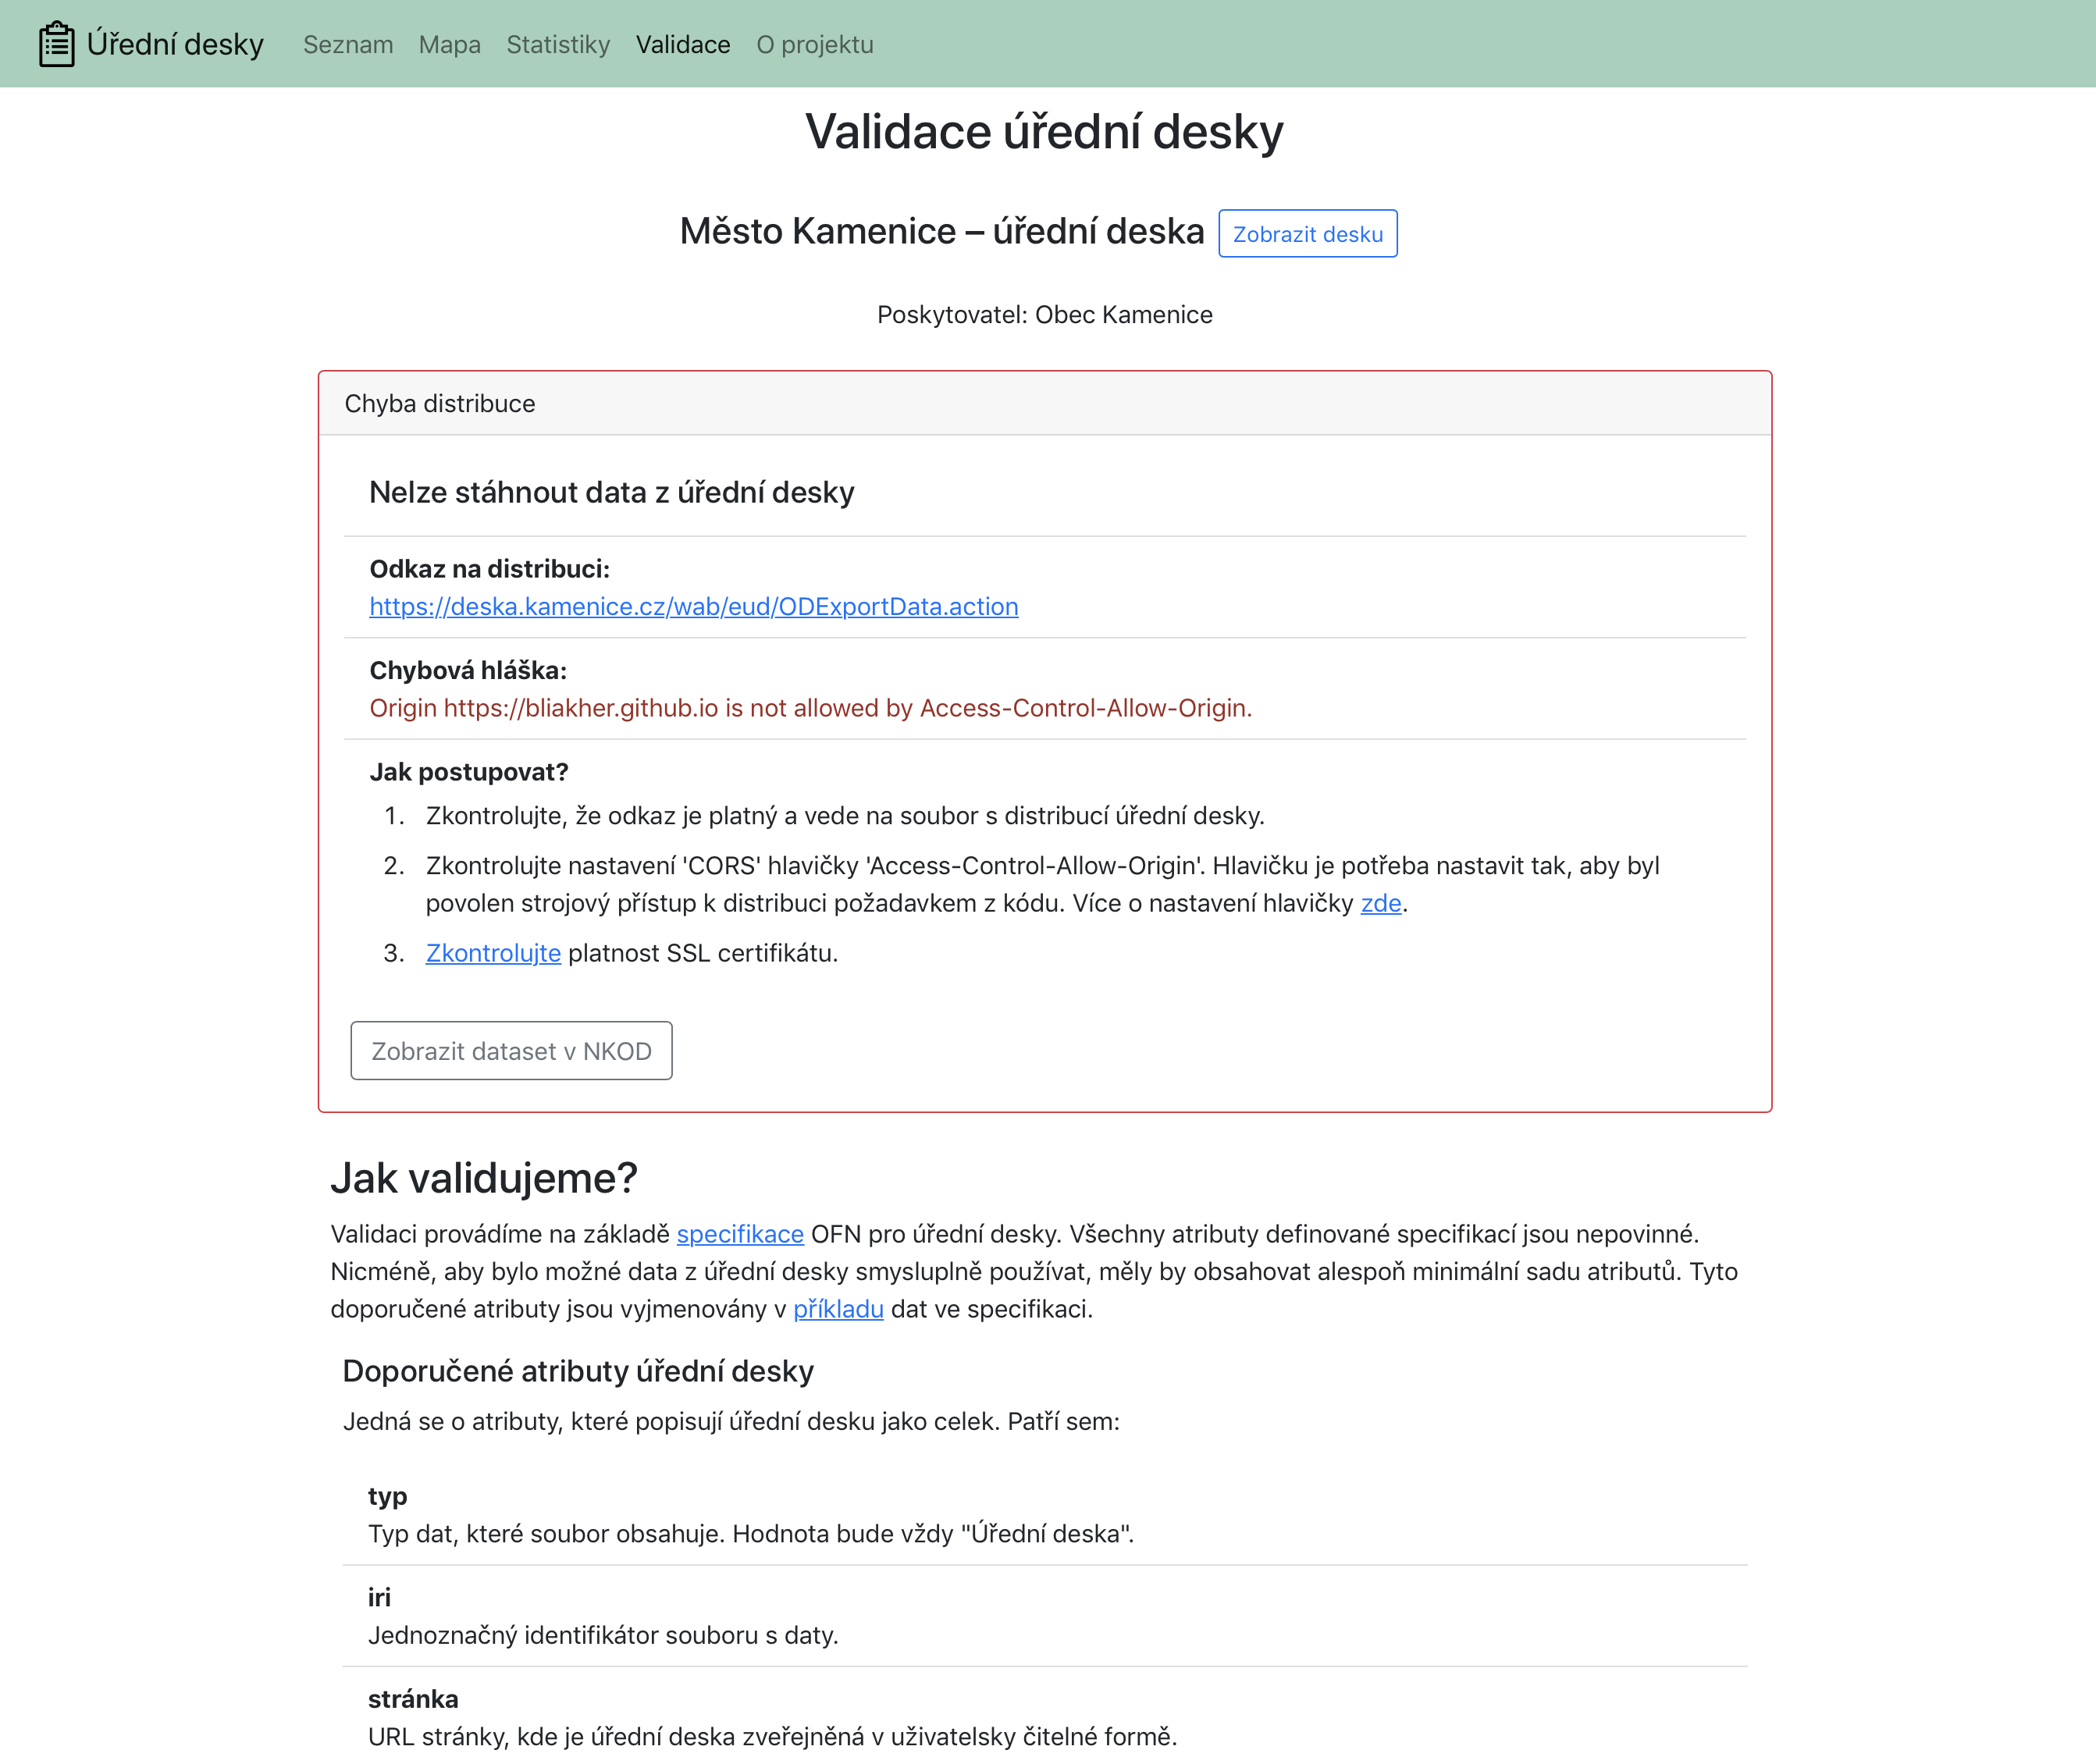
\includegraphics[width=\textwidth]{cs/obrazky/screenshots/validace_detail_cerveny.png}
\caption{Ukázka detailu validace úřední desky, u které není možné stáhnout distribuci}
\label{fig:screen-validace-c}
\end{figure}

Pokud v distribuci desky chybí některé doporučené atributy, je zde
vypsané, které to jsou. Pokud se jedná o doporučené atributy informací,
zobrazí se v záložce \textit{Informace\ s\ chybějícími\ atributy} seznam
všech informací s nedostatky, kde u každé informace je uvedeno, které
atributy chybí.

Na následujícím příkladu (\autoref{fig:screen-validace-z}) validace desky úřadu městské části Praha 5 si
můžeme všimnout, že v distribuci chybí doporučený atribut desky
\texttt{provozovatel} a v 10 informacích na desce z celkem 144 chybí
doporučený atribut \texttt{relevantní\_do}. Můžeme si prohlédnout, o
které informace se jedná.

\begin{figure}
\centering
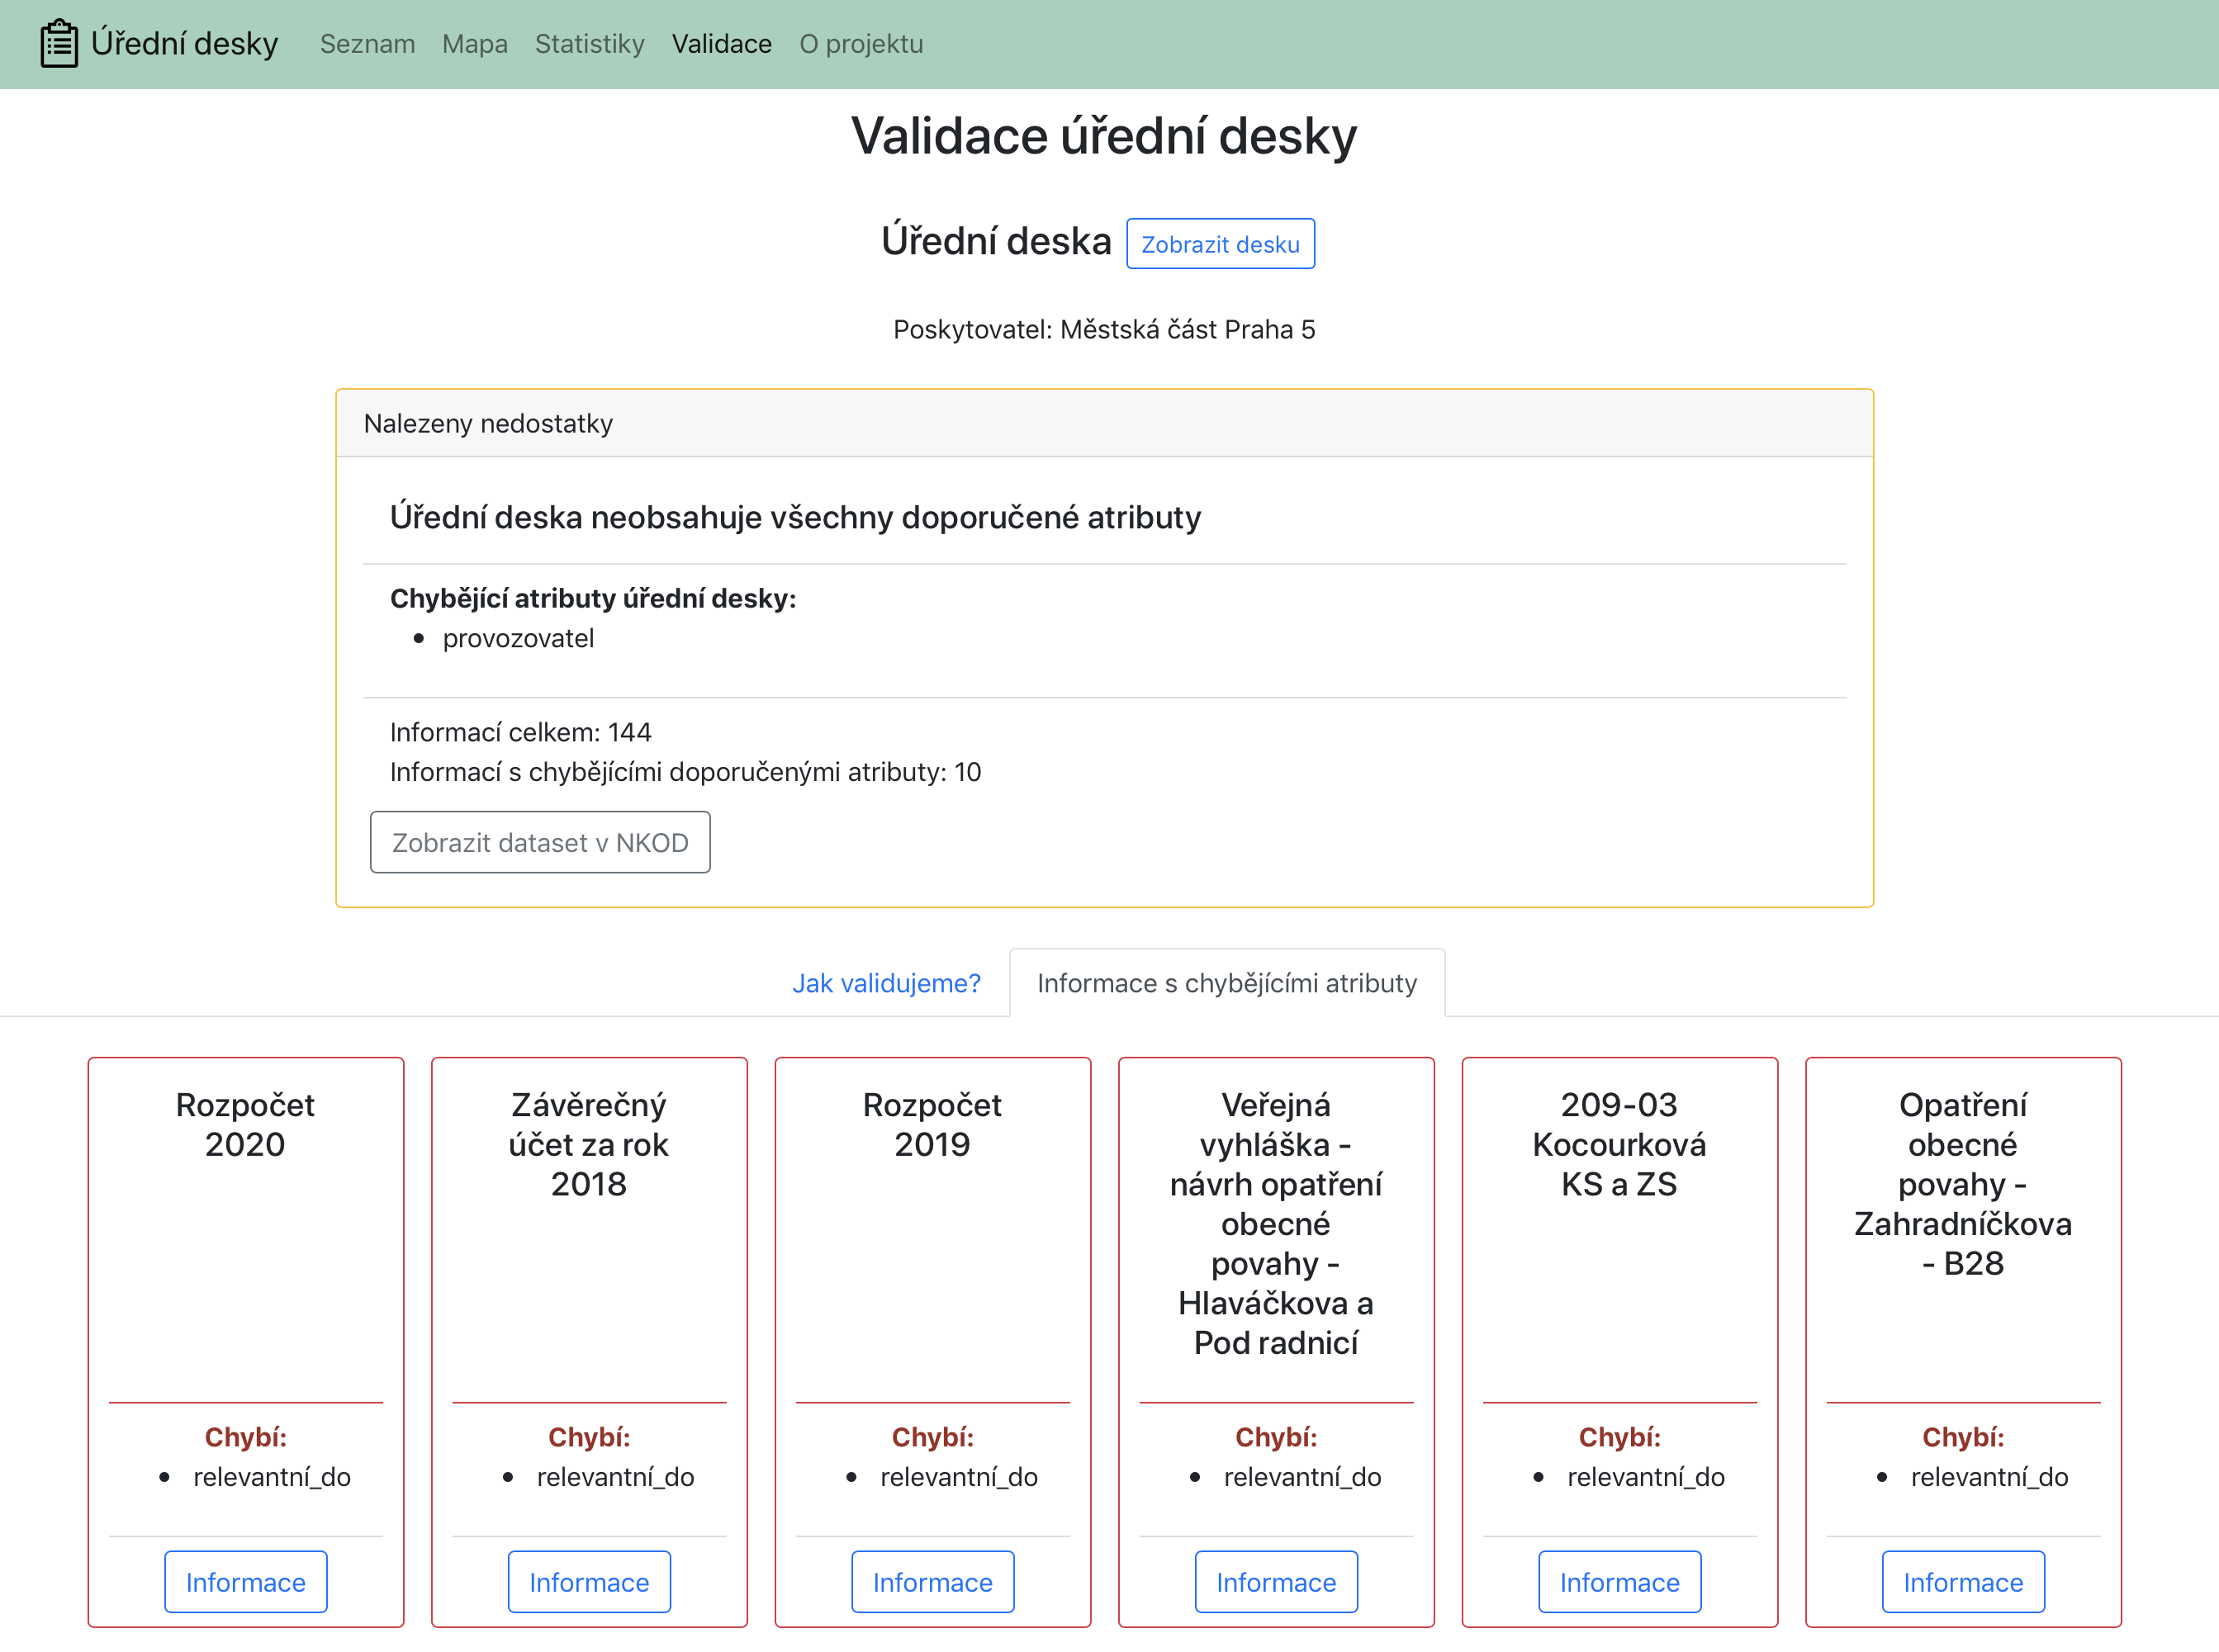
\includegraphics[width=\textwidth]{cs/obrazky/screenshots/validace_detail_zluty.png}
\caption{Ukázka detailu validace úřední desky, u které chybí některé doporučené atributy}
\label{fig:screen-validace-z}
\end{figure}

\subsection*{Statistiky}\label{statistiky}

V této části se zobrazují souhrnné statistiky výsledků validace a
poskytovatelů. Část Statistiky je rozdělená na 2 záložky --- \textit{Validace} a \textit{Poskytovatelé}.

V záložce \textit{Validace} jsou zobrazeny souhrnné výsledky validace v textové podobě a na koláčovém grafu. Jsou zde také seznamy desek, které obsahují nedostatky, ze kterých je možné se prokliknout na detail jejich validace.

Příklad validační statistiky vidíme na obrázku \ref{fig:screen-stat-val}.

\begin{figure}
\centering
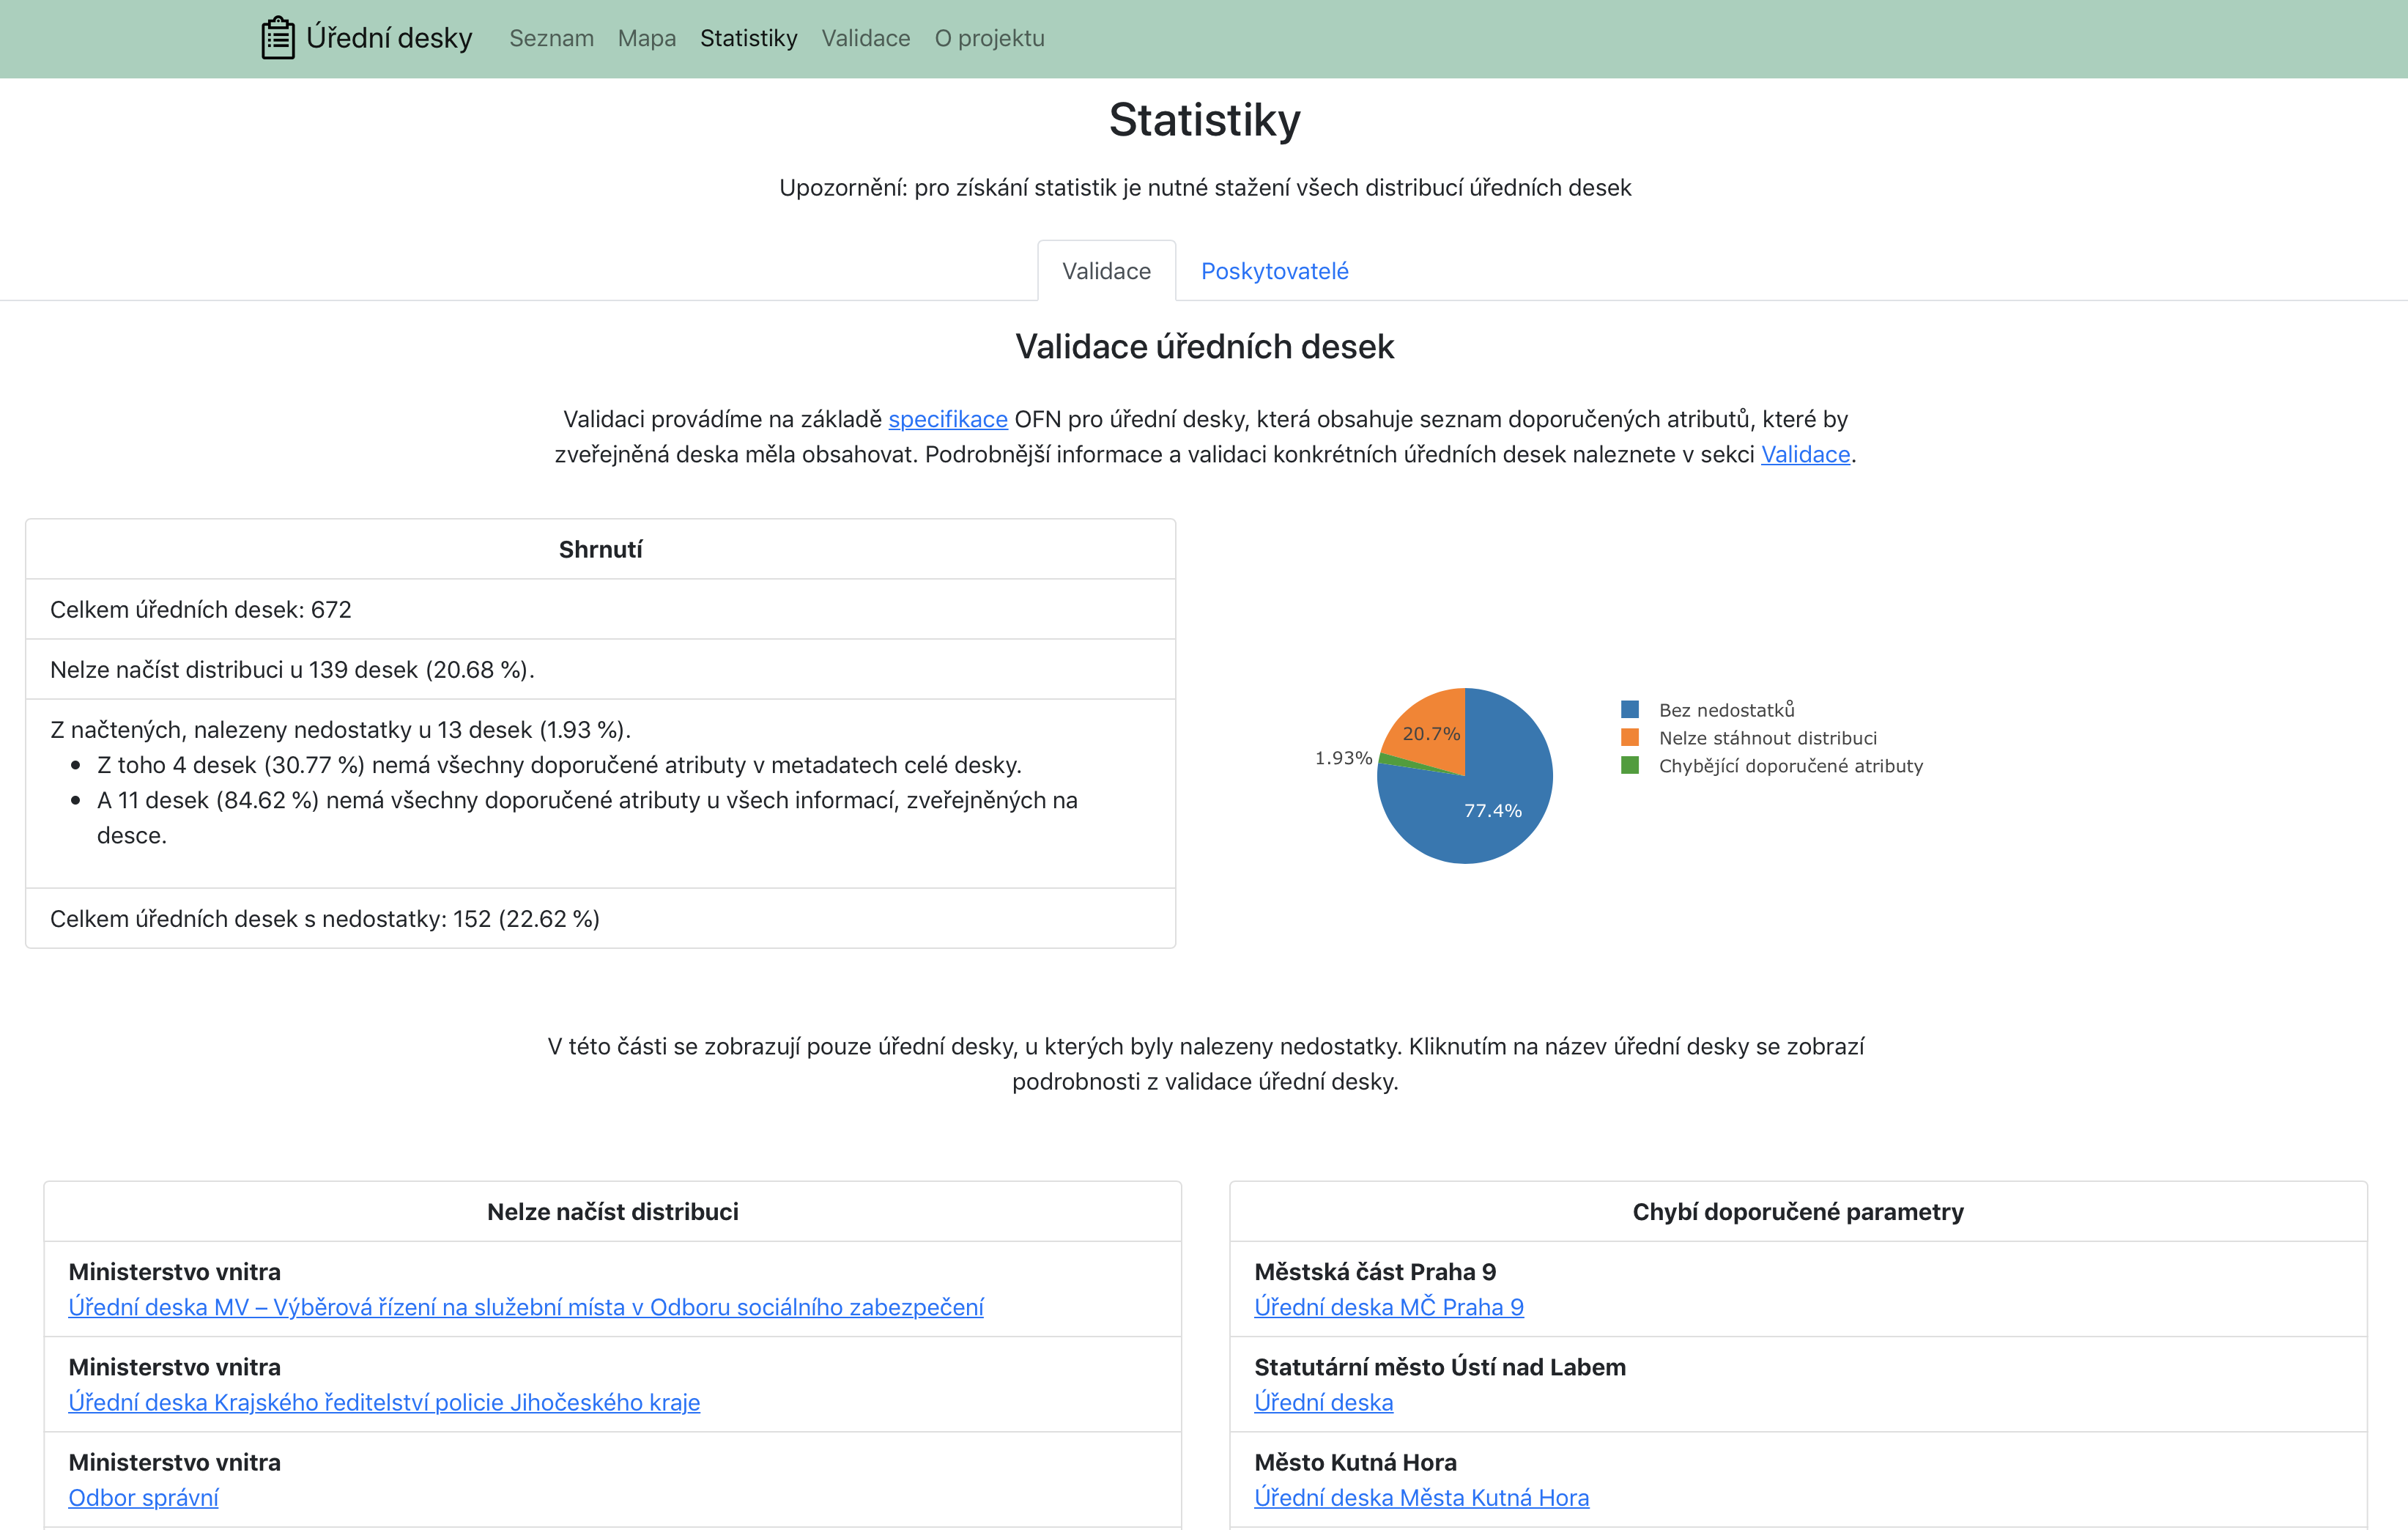
\includegraphics[width=\textwidth]{cs/obrazky/screenshots/statistika_validace.png}
\caption{Ukázka validační statistiky}
\label{fig:screen-stat-val}
\end{figure}

V záložce \textit{Poskytovatelé} je statistika poskytovatelů. Je zde zobrazeno, pro jednotlivé právní formy, kolik je celkem orgánů dané právní formy a kolik z nich poskytuje data ze svých úředních desek jako otevřená data. Pro největší skupiny poskytovatelů je toto zobrazeno na koláčových grafech a pro ostatní skupiny v textovém seznamu.

\begin{figure}
\centering
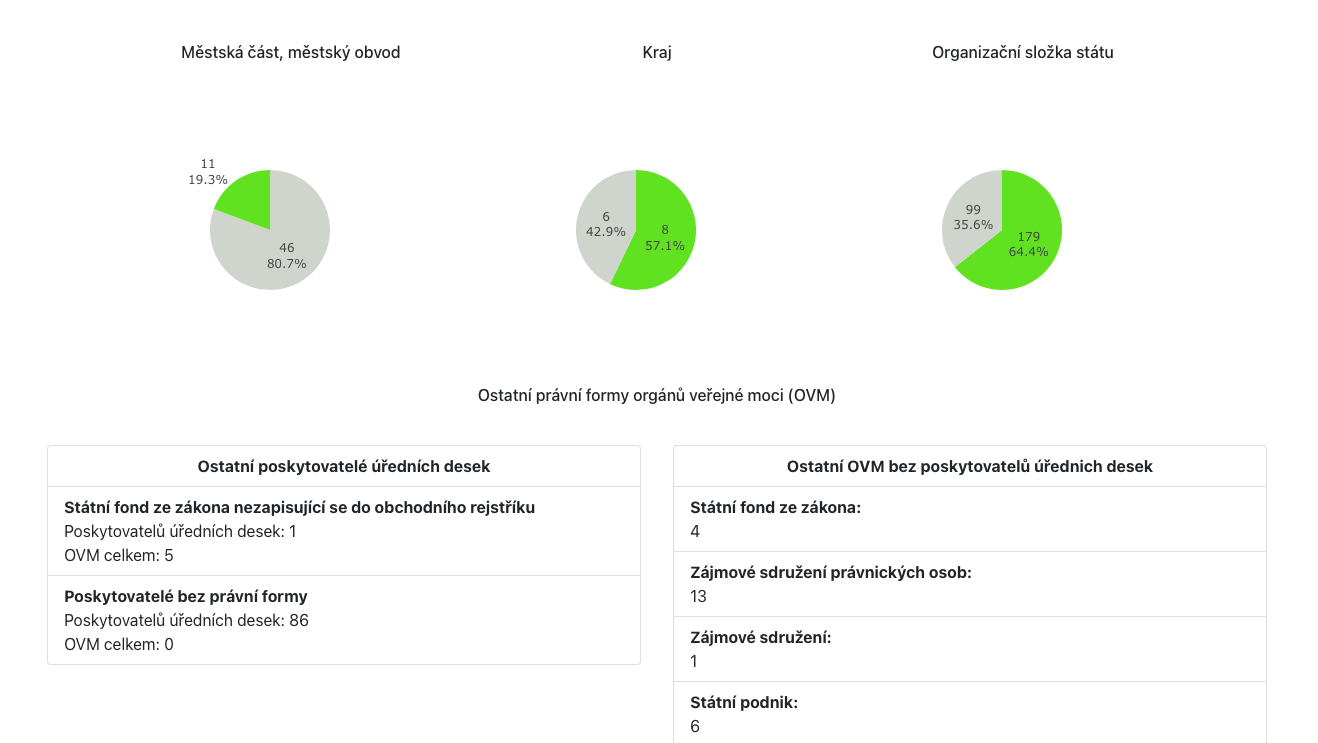
\includegraphics[width=\textwidth]{cs/obrazky/screenshots/statistika_poskytovatele.png}
\caption{Ukázka statistiky poskytovatelů}
\label{fig:screen-stat-posk}
\end{figure}

Na obrázku \ref{fig:screen-stat-posk} vidíme část statistiky poskytovatelů, konkrétně grafy pro městské
části, kraje a organizační složky státu. Pod nimi jsou 2 seznamy, v
prvním jsou poskytovatelé ostatních právních forem. Můžeme si všimnout,
že pro 86 poskytovatelů se nepodařilo zjistit jejich právní formu, což
nejspíše znamená, že tito poskytovatelé nemají svoji právní formu
uvedenou v
\href{https://www.szrcr.cz/cs/registr-prav-a-povinnosti}{Registru práv a
povinností}, odkud data o poskytovatelích získáváme.

Ve druhém seznamu jsou právní formy, které nemají žádného poskytovatele
úředních desek. U každé formy je uvedený celkový počet orgánů této
právní formy.


\section{Vývojářská dokumentace}\label{sec:developer-docs}

Vývojářská dokumentace je dostupná online na \url{https://bliakher.github.io/uredni_desky_docs/vyvojarska/}.

Vývojářská dokumentace obsahuje adresářovou strukturu repozitáře, popis vzájemného fungování různých částí aplikace a popis vybraných tříd a rozhraní. Je zde možné najít také dokumentaci všech tříd a rozhraní v aplikaci, vygenerovanou z komentářů v kódu pomocí nástroje TypeDoc \footnote{\url{https://typedoc.org/}}.


\section{Administrátorská dokumentace}\label{sec:admin-docs}

Administrátorská dokumentace je dostupná online na \url{https://bliakher.github.io/uredni_desky_docs/administratorska/}.

Obsahuje seznam požadavků a instrukce pro sestavení a nasazení aplikace.
